\documentclass[t]{beamer}
\usetheme[deutsch]{KIT}
\setbeamercovered{transparent}
\setbeamertemplate{navigation symbols}{}

\KITfoot{Tutoriumsmaterial von Alexander Kwiatkowski, Michael Vollmer und Matthias Holoch \hspace{2.5cm} Basierend auf den Folien von Simon Stroh und Moritz v. Looz}
\usepackage[utf8]{inputenc}
\usepackage{amsmath}
\usepackage{ifthen}
\usepackage{amssymb}
\usepackage{tikz}
\usepackage{ngerman}
\usepackage[normalem]{ulem}
\usetikzlibrary{automata}
\usenavigationsymbols


\title{Theoretische Grundlagen der Informatik}
\subtitle{Tutorium}
\author{Alexander Kwiatkowski, Michael Vollmer und Matthias Holoch}

\institute[IKS]{Institut für Kryptographie und Sicherheit}

\TitleImage[height=\titleimageht]{images/tmaschine.png}

\newcommand{\N}{\ensuremath{\mathbb{N}}}
\newcommand{\M}{\ensuremath{\mathcal{M}}}
\newcommand{\classP}{\ensuremath{\mathcal{P}}}
\newcommand{\classNP}{\ensuremath{\mathcal{NP}}}
\newcommand{\co}{\ensuremath{\mathsf{co\text{-}}}}
\newcommand{\pot}{\ensuremath{\mathcal{P}}}
\newcommand{\abs}[1]{\ensuremath{\left\vert #1 \right\vert}}
\newcommand{\menge}[2]{\ensuremath{\left\lbrace #1 \,\middle\vert\, #2 \right\rbrace}}
\newcommand{\ducttape}[1]{\vspace{#1}}
\newcommand{\neglit}[1]{\overline{#1\vphantom{x^a}}}
\newcommand{\recipe}{\raisebox{-.3cm}{
\includegraphics[scale=.15]{images/chefs-cap.png}}\hspace{0.2cm}}
\newcommand{\opt}[1]{\ensuremath{\text{OPT}(#1)}}
\newcommand{\A}[1]{\ensuremath{\mathcal{A}(#1)}}
\renewcommand{\O}[1]{\ensuremath{\mathcal{O}(#1)}}
\newcommand{\msout}[1]{\text{\sout{\ensuremath{#1}}}}

\newcommand{\invincible}{\setbeamercovered{invisible}} %  "Yesss! I am invincible!!" (Boris Grishenko)
\newcommand{\vincible}{\setbeamercovered{transparent}}
\renewcommand{\solution}[1]{\invincible \pause #1 \vincible}
\newcommand{\micropause}{\\[8pt]}

% \@ifundefined{tikzset}{}{\tikzset{initial text=}} % Text "start" bei Startknoten unterdrücken
\tikzstyle{every node}=[thick]
\tikzstyle{every line}=[thick]

\newcommand{\tutnr}[1]{
  \subtitle{Tutorium #1}
	\begin{frame}
		\maketitle
	\end{frame}
}

\newcommand{\uebnr}[1]{
  \subtitle{Anmerkungen zum #1. Übungsblatt}
	\begin{frame}
		\maketitle
	\end{frame}
}

\begin{document}

\tutnr{1}
\newcommand{\start}[3]
{
  \draw (#1*2,#2*2) node{$#3$};
  \draw (#1*2,#2*2) circle(0.4cm);
  \draw [->] (#1*2-0.9,#2) -- (#1*2-0.4,#2);
}
\newcommand{\state}[3]
{
  \draw (#1*2,#2*2) node{$#3$};
  \draw (#1*2,#2*2) circle(0.4cm);
}
\newcommand{\final}[3]
{
  \draw (#1*2,#2*2) node{$#3$};
  \draw (#1*2,#2*2) circle(0.4cm);
  \draw (#1*2,#2*2) circle(0.32cm);
}
\newcommand{\tol}[4]
{
  \draw (#1+#3,#2*2) node[above]{$#4$};
  \draw [->] (#1*2-0.4,#2*2) -- (#3*2+0.4,#2*2);
}
\newcommand{\tor}[4]
{
  \draw (#1+#3,#2*2) node[above]{$#4$};
  \draw [->] (#1*2+0.4,#2*2) -- (#3*2-0.4,#2*2);
}
\newcommand{\tot}[4]
{
  \draw (#1*2,#2+#3) node[right]{$#4$};
  \draw [->] (#1*2,#2*2+0.4) -- (#1*2,#3*2-0.4);
}
\newcommand{\tob}[4]
{
  \draw (#1*2,#2+#3) node[right]{$#4$};
  \draw [->] (#1*2,#2*2-0.4) -- (#1*2,#3*2+0.4);
}
\newcommand{\totl}[5]
{
  \draw (#1+#3,#2+#4) node[above right]{$#5$};
  \draw [->] (#1*2-0.283,#2*2+0.283) -- (#3*2+0.283,#4*2-0.283);
}
\newcommand{\totr}[5]
{
  \draw (#1+#3,#2+#4) node[above left]{$#5$};
  \draw [->] (#1*2+0.283,#2*2+0.283) -- (#3*2-0.283,#4*2-0.283);
}
\newcommand{\tobl}[5]
{
  \draw (#1+#3,#2+#4) node[below right]{$#5$};
  \draw [->] (#1*2-0.283,#2*2-0.283) -- (#3*2+0.283,#4*2+0.283);
}
\newcommand{\tobr}[5]
{
  \draw (#1+#3,#2+#4) node[below left]{$#5$};
  \draw [->] (#1*2+0.283,#2*2-0.283) -- (#3*2-0.283,#4*2+0.283);
}
\newcommand{\rloopl}[3]
{
  \draw (#1*2-1,#2*2) node[left]{$#3$};
  \draw [->] (#1*2-0.35,#2*2-0.2) arc (-30:-320:0.32cm);
}
\newcommand{\rloopr}[3]
{
  \draw (#1*2+1,#2*2) node[right]{$#3$};
  \draw [->] (#1*2+0.35,#2*2+0.2) arc (150:-140:0.32cm);
}
\newcommand{\rloopt}[3]
{
  \draw (#1*2,#2*2+1) node[above]{$#3$};
  \draw [->] (#1*2-0.2,#2*2+0.35) arc (240:-50:0.32cm);
}
\newcommand{\rloopb}[3]
{
  \draw (#1*2,#2*2-1) node[below]{$#3$};
  \draw [->] (#1*2+0.2,#2*2-0.35) arc (60:-230:0.32cm);
}
\newcommand{\lloopl}[3]
{
  \draw (#1*2-1,#2*2) node[left]{$#3$};
  \draw [->] (#1*2-0.35,#2*2+0.2) arc (30:320:0.32cm);
}
\newcommand{\lloopr}[3]
{
  \draw (#1*2+1,#2*2) node[right]{$#3$};
  \draw [->] (#1*2+0.35,#2*2-0.2) arc (-150:140:0.32cm);
}
\newcommand{\lloopt}[3]
{
  \draw (#1*2,#2*2+1) node[above]{$#3$};
  \draw [->] (#1*2+0.2,#2*2+0.35) arc (-60:230:0.32cm);
}
\newcommand{\lloopb}[3]
{
  \draw (#1*2,#2*2-1) node[below]{$#3$};
  \draw [->] (#1*2-0.2,#2*2-0.35) arc (-240:50:0.32cm);
}
\section{Organisatorisches}

\subsection{Organisatorisches}

\begin{frame}
	\frametitle{\texttt{whois tutor}}
	
	\begin{itemize}
		\item \textbf{Alexander Kwiatkowski} \\ alexander.kwiatkowski@gmx.net \\ Dienstag 17:30, SR -120
		\item \textbf{Michael Vollmer} \\ Michael@trollbu.de \\ Dienstag 17:30, SR -119
		\item \textbf{Matthias Holoch} \\ Matthias.Holoch@student.kit.edu \\ Donnerstag 8:00, SR -120
	\end{itemize}
\end{frame}

\begin{frame}
	\frametitle{Organisatorisches -- Zum Übungsbetrieb}
	\begin{itemize}
		\item \textbf{Abgabe:} \emph{Handschriftlich} in Gruppen
		\begin{itemize}
			\item Bis zu 5 Personen pro Gruppe
			\item Erste Abgabe legt die Gruppe fest
			\item Jede Person muss ein eigenes Blatt abgeben (mit Gruppenname falls vorhanden)
		\end{itemize}
		\item \textbf{Schein:} 
		\begin{itemize}
			\item Klausurbonus (1 Notenschritt)
			\item Bei min. 6 (von 7) Blättern 50\% Punkte
		\end{itemize}
		\item korrigierte Übungsblätter gibt es im Tutorium
		\begin{itemize}
			\item Bei Nichtabholung: Büro 274 Montags 14:00-15:00
		\end{itemize}
	\end{itemize}
\end{frame}
\begin{frame}
	\frametitle{Organisatorisches -- Zum Tutorium}
	\begin{itemize}
	\item Tutoriumsfolien
		\begin{itemize}
			\item \texttt{http://tinyurl.com/tgi1213}
		\end{itemize}
		\item E-Mail-Liste geht rum
		\item Stoff soll wiederholt werden
		\item Dabei Fokus auf Übungsbetrieb
		\item Fragen/Vorschläge/Anmerkungen willkommen!
	\end{itemize}
\end{frame}
\section{Endliche Automaten}
\subsection{Deterministische endliche Automaten}
\begin{frame}
\frametitle{Deterministische endliche Automaten}

	\begin{minipage}{0.5 \textwidth}
	 \raggedright{ Ein deterministischer endlicher Automat $M$ ist ein 5-Tupel 
        \[
        M= (Q,\Sigma,\delta,s,F).
        \] }
        \begin{itemize}
        \item $Q$:  endliche Zustandsmenge
        \item $\Sigma$:    endliches Alphabet
        \item $\delta$:   Zustandsübergangsfunktion $Q\times \Sigma \rightarrow Q$
        \item $s$:   Startzustand $\in Q$
        \item $F$:   Endzustandsmenge $\subseteq Q$
        \end{itemize}
	\end{minipage}
	\hfill
    \begin{minipage}{0.45 \textwidth}        
        \begin{center}
        	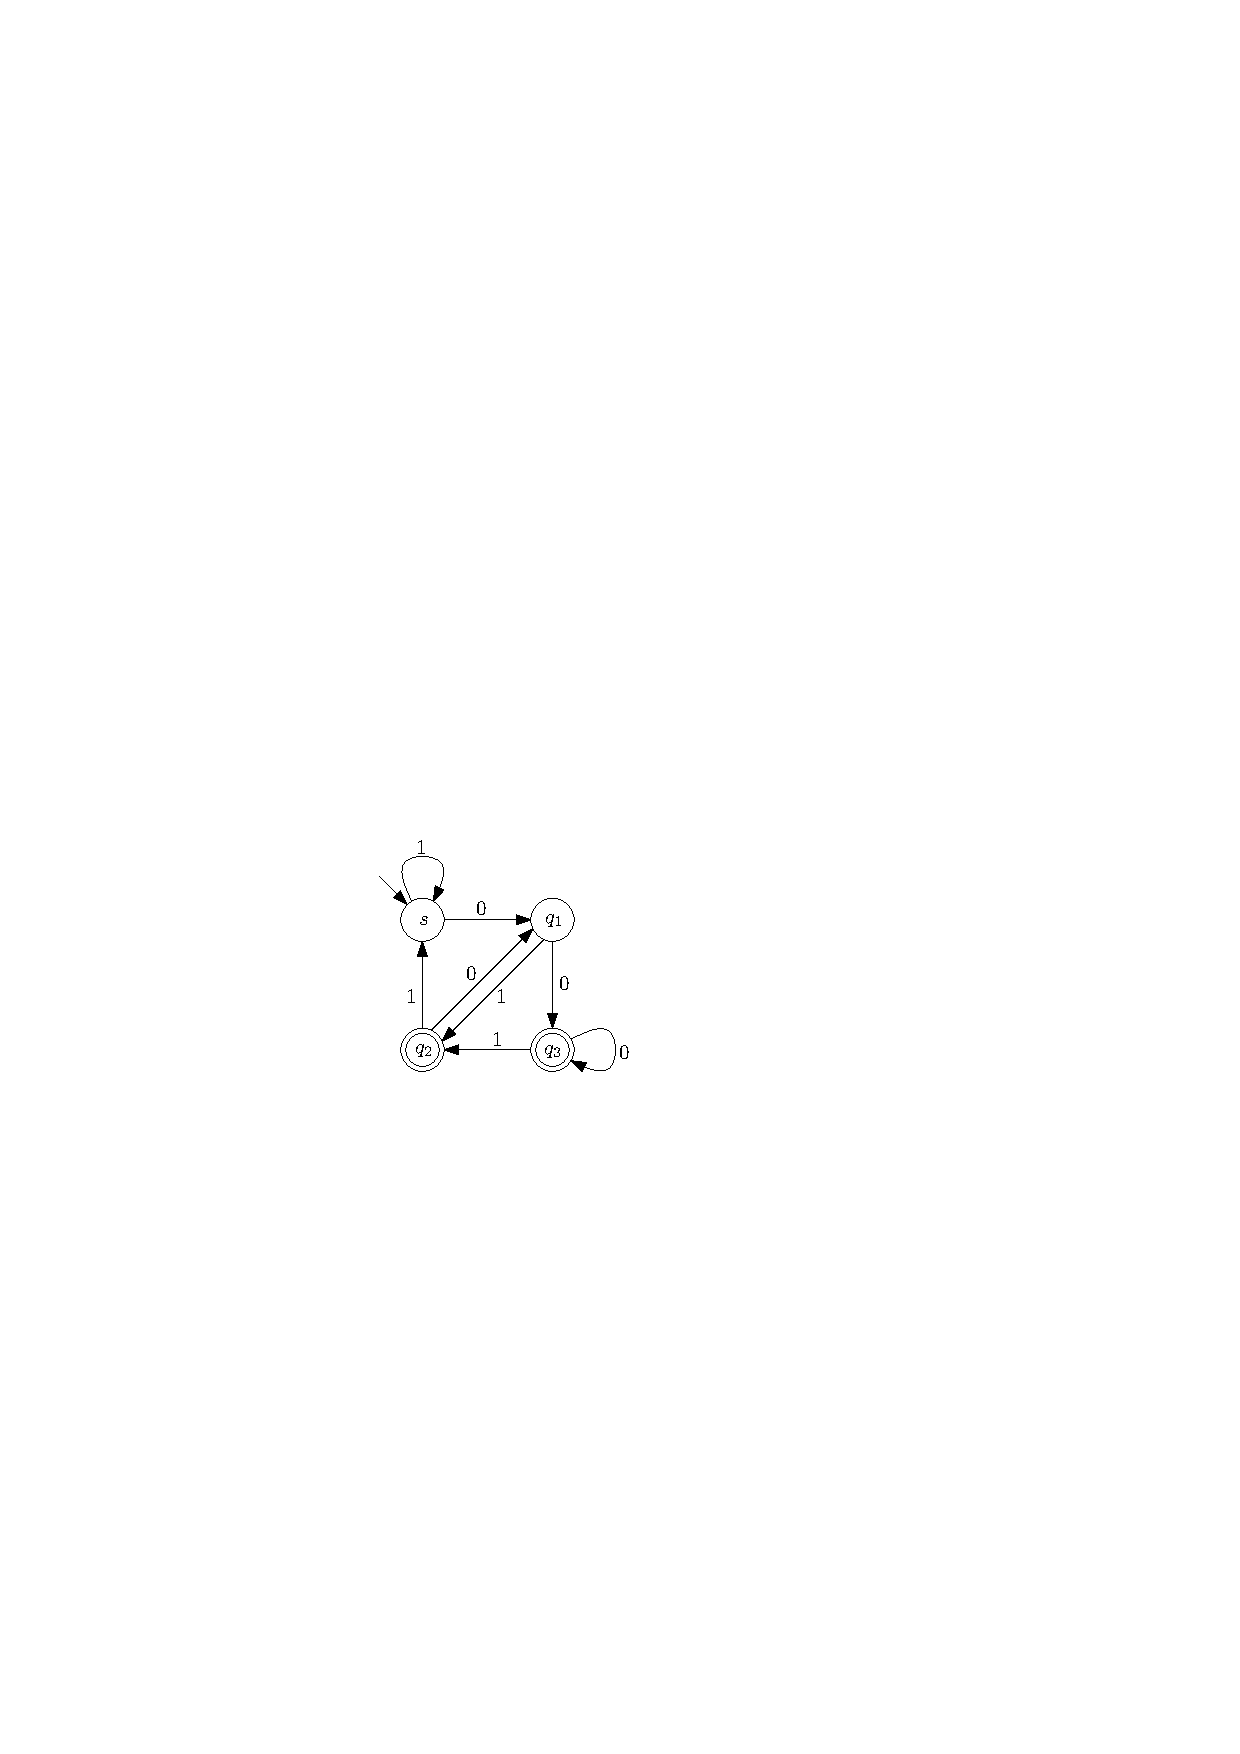
\includegraphics[scale=1]{images/beispielDEA1.pdf}
        \end{center}
    \end{minipage}
\end{frame}
%\begin{frame}
%	\frametitle{DEA: Aufgaben}
%	\begin{enumerate}
%	\item 
%		Lösen Sie folgendes Rätsel mit Hilfe eines deterministischen
%		endlichen Automaten:
%		\begin{quote}
%		  Es stehen drei Wasserkrüge mit einem Fassungsvermögen
%		  von 3, 5 bzw. 7 $l$ zur Verfügung, um eine Wassermenge von
%		  einem Liter abzumessen, d.~h. in einem der Krüge soll sich genau
%		  diese Menge Wassers befinden. Zu Beginn sind der kleinste und
%		  der größte Krug gefüllt. Da Ihr Augenmaß schlecht
%		  ist, darf Wasser nur so von einem Krug in einen anderen
%		  gegossen werden, dass der eine ganz geleert oder der andere
%		  ganz gefüllt wird (ohne dass Wasser verschüttet wird).
%		\end{quote}
%		Geben Sie den Übergangsgraphen eines Automaten an, dessen
%		akzeptierte Sprache genau die zulässigen lösenden
%		Umfüllreihenfolgen kodiert, sowie ein kürzestes Lösungswort.
%	\end{enumerate}
%\end{frame}
%\begin{frame}
%\frametitle{DEA: Aufgabe}
%\begin{enumerate}
%\setcounter{enumi}{1}
%\item Geben Sie einen regulären Ausdruck für die vom DEA mit nachfolgendem Zustandsgraphen erkannte Sprache an:
%\begin{center}
%\begin{tikzpicture}[node distance=2cm,shorten >=1pt,auto]
%\node[state,initial,initial where=above]   (q_0)                {$q_0$};
%\node[state]           (q_1) [left of=q_0]  {$q_1$};
%\node[state,accepting] (q_2) [below of=q_0] {$q_2$};
%\node[state,accepting] (q_3) [left of=q_2]  {$q_3$};
%\path[->]	(q_0) 	edge 			node {$b$} 		(q_2)
%			edge 			node {$c$} 		(q_1)
%			edge 			node {$a$} 		(q_3)
%		(q_1)	edge [loop above]	node {$a$,$b$,$c$}	()
%		(q_2)	edge [bend left]	node {$a$}		(q_3)
%			edge [bend left=90,looseness=2.2]	node {$b$,$c$}		(q_1)
%		(q_3)	edge			node {$a$,$c$}		(q_1)
%			edge			node {$b$}		(q_2);
%\end{tikzpicture}
%\end{center}
%\end{enumerate}
%\end{frame}
%\begin{frame}
%	\begin{enumerate}
%	\setcounter{enumi}{2}
%	\item Aufgabe: Konstruiere einen DEA, der alle durch 5 teilbaren Zahlen akzeptiert. Als Eingabe erhält der Automat dabei die Zahl in ihrer binären Darstellung. Also ist $\Sigma = \{0, 1\}$. Z.B. soll Automat $10_{10} = 1010_{2}$ akzeptieren, aber $7_{10} = 111_{2}$ ablehnen.
%	\pause \\[10pt]
%	Tip: Restklassen als Zustände modellieren
%	\end{enumerate}
%\end{frame}
%\begin{frame}
%	\frametitle{DEA: Lösung}
%	\begin{enumerate}
%	\setcounter{enumi}{2}
%	\item Idee
%		\begin{itemize}
%		\item $Q = (q_0, q_1, q_2, q_3, q_4)$\\
%		\item $\Sigma = \{0,1\}$
%		\item $\delta(q_n, c) = q_{n \cdot 2 + c\mbox{ mod }5}$ mit $c\in\Sigma$\\
%		\item $s = q_0$\\
%		\item $F = \{q_0\}$
%		\end{itemize}
%	\end{enumerate}
%\end{frame}
\subsection{Nichtdeterministische endliche Automaten}
\begin{frame}
\frametitle{Nichtdeterministische endliche Automaten}

	\begin{minipage}{0.5 \textwidth}
        Ein nichtdeterministischer endlicher Automat $M$ ist ein 5-Tupel
        \[
        M= (Q,\Sigma,\delta,s,F).
        \]
        \begin{itemize}
        \item $Q$:  endliche Zustandsmenge
        \item $\Sigma$:    endliches Alphabet
        \item \textcolor{red}{$\delta$:   Zustandsübergangsfunktion $Q\times (\Sigma \cup \varepsilon) \rightarrow \pot(Q)$}
        \item $s$:   Startzustand $\in Q$
        \item $F$:   Endzustandsmenge $\subseteq Q$
        \end{itemize}
\vspace{0.5cm}
	Damit der NEA ein Wort akzeptiert, muss es \emph{einen} akzeptierenden Weg geben.
	
	\end{minipage}
	\hfill
    \begin{minipage}{0.45 \textwidth}        
        \begin{center}
        	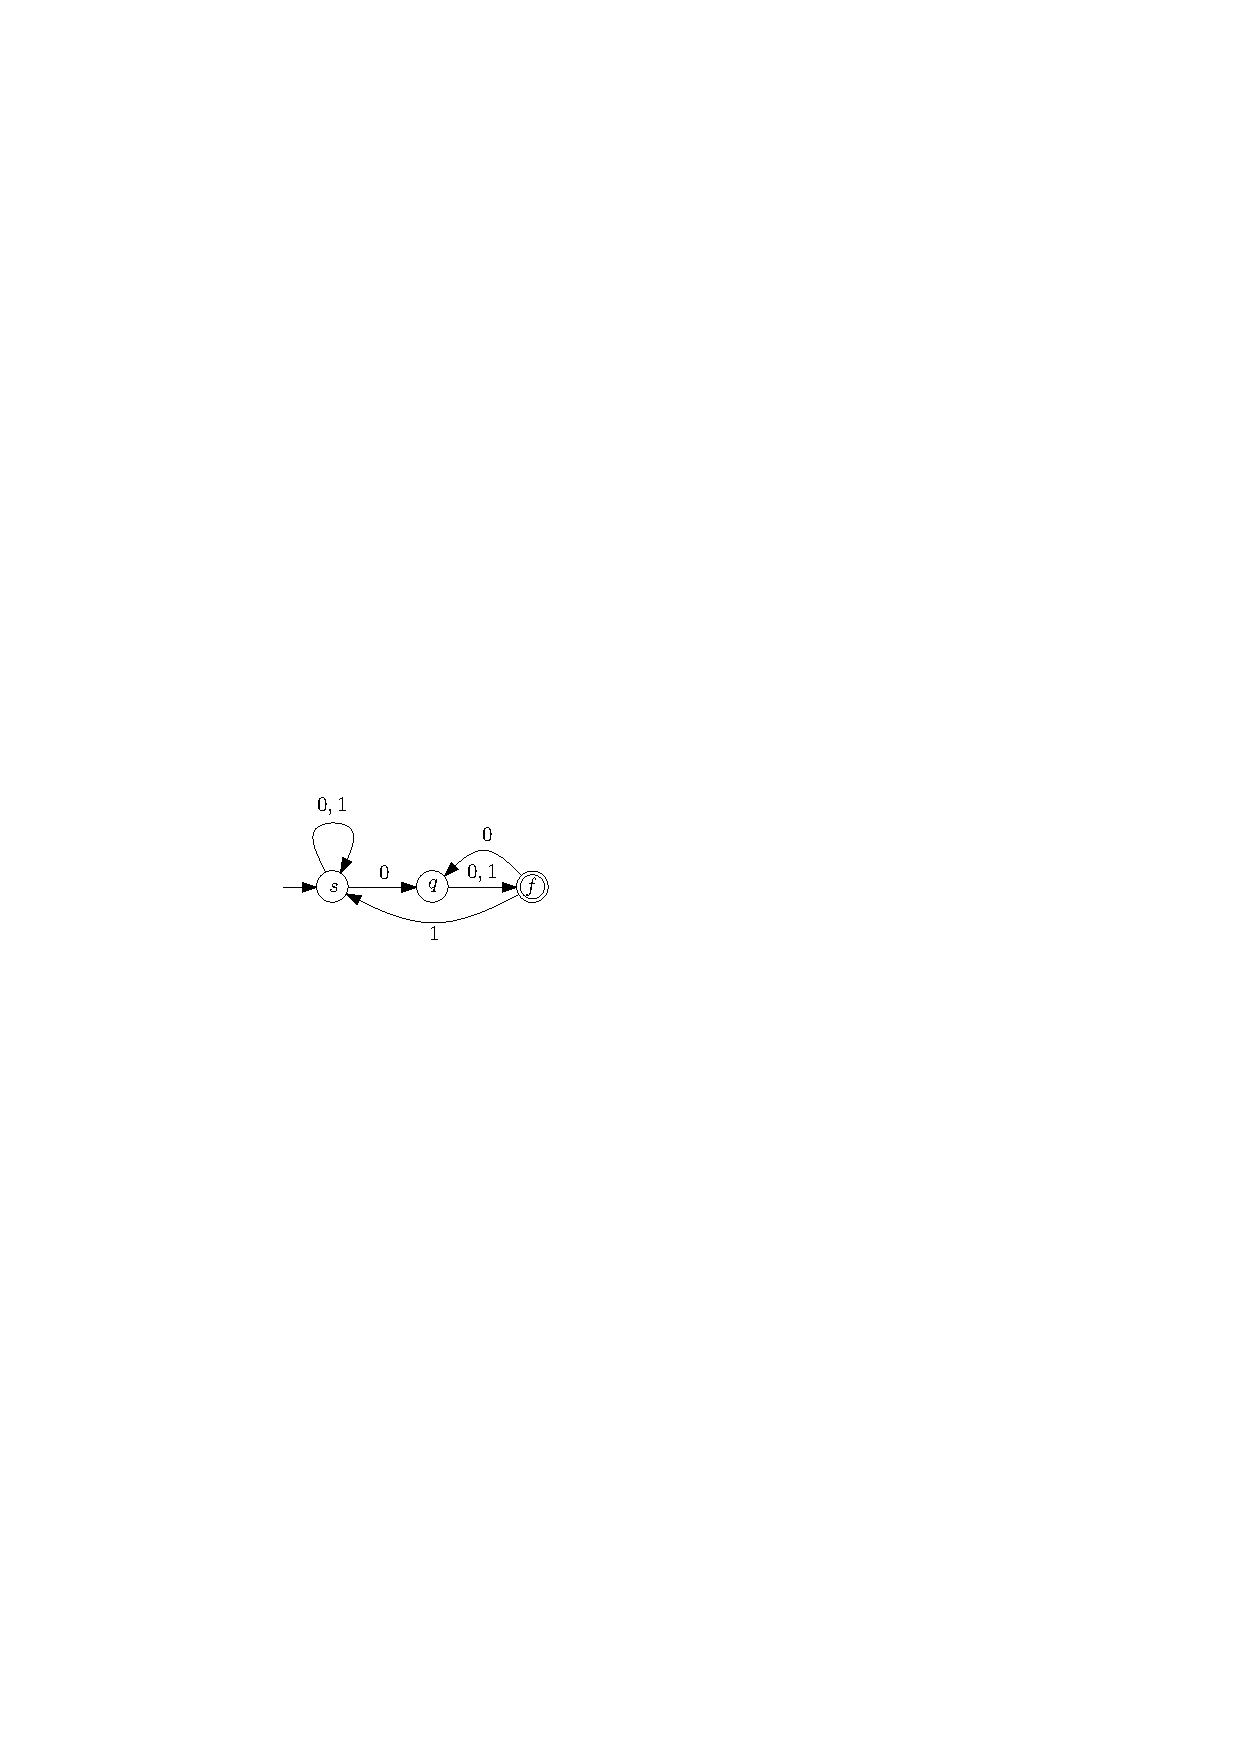
\includegraphics[scale=1]{images/beispielNEA.pdf}
        \end{center}
    \end{minipage}
\end{frame}
\begin{frame}
	\frametitle{NEA: Beispiel}
	\begin{figure}
	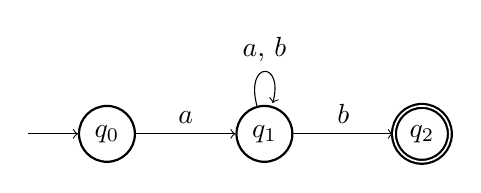
\begin{tikzpicture}
	\node[draw,circle] (q_0) at (0,0) {$q_0$};
	\node[draw,circle] (q_1) at (2,0) {$q_1$};
	\node[draw,circle,double] (q_2) at (4,0) {$q_2$};
	\draw[->] (-1,0) -- (q_0);
	\draw[->] (q_0) -- (q_1) node[midway,anchor=south] {$a$};
	\draw[->] (q_1) -- (q_2) node[midway,anchor=south] {$b$};
	\draw (q_1) edge [loop above] node {$a$, $b$} (q_1);
	\end{tikzpicture}
	\end{figure}
 	Bei Eingabe von $b$ im Zustand $q_1$ gibt es mehrere Möglichkeiten. \vspace{0.5cm}
	
	(siehe Berechnungsbaum an der Tafel).
\end{frame}

\section{Reguläre Sprachen}
\subsection{Reguläre Sprachen}
\begin{frame}
\frametitle{Rechtslineare Grammatiken}
Eine Grammatik $G = ( T, V, S, P)$
\begin{itemize}
	\item $T$ = Menge der Terminale (a.k.a. Alphabet der Sprache)
	\item $V$ = Menge der Nichtterminale (zu T disjunkt)
	\item $S \in V$ = Startsymbol
	\item $P \subset V^{+} \times (V \bigcup T)^{*}$ = Menge der Produktionen
\end{itemize}
bei der alle Produktionen so aussehen:
\begin{itemize}
	\item $A \rightarrow \lambda$
	\begin{itemize}
		\item $A \in V$
		\item $\lambda$ ist leeres Wort
	\end{itemize}
	\item $A \rightarrow bC$
	\begin{itemize}
		\item $A, C \in V$
		\item $b \in T$
	\end{itemize}
\end{itemize}
heißt rechtslinear bzw. regulär. 
\end{frame}

\begin{frame}
\frametitle{Reguläre Ausdrücke}
$A$ ist ein regulärer Ausdruck über dem Alphabet $\Sigma$ wenn:
\begin{itemize}
	\item $A = \lambda$
	\item $A = x \in \Sigma$
	\item $A = B^{*} = \{\lambda, B, BB, BBB, \ldots\}$
	\item $A = B^{+} = \{B, BB, BBB, \ldots\}$
	\item $A = B \cdot C = \{BC\}$
	\item $A = B + C = \{B, C\}$
\end{itemize}
Wobei B und C ebenfalls reguläre Ausdrücke über $\Sigma$ sind.
~\\~\\~\\~\\

Bitte deutlich schreiben:
\begin{equation*}
B^{+}C \neq B + C
\end{equation*}
\end{frame}

\subsection*{Aufgabe 1}
\begin{frame}
	\frametitle{Aufgabe 1}
	\only<1>{
	Gegeben sei der folgende endliche Automat:\\
	$\mathcal{M} = (\mathcal{Q},\Sigma,\delta,S,\mathcal{F})$ mit
	$\Sigma = \{a,b\}$, $\mathcal{Q} = \{S,B,C,D\}$, $\mathcal{F} = \{B,C\}$
	und $\delta$ gegeben durch:
	}
	\only<2>{\vspace{-1.7 cm}}
	\begin{center}
		\resizebox{4cm}{!} {%
		\begin{tikzpicture}[line width=1pt]
			\start{0}{0}{S}
			\totr{0}{0}{1}{1}{a}
			\tobr{0}{0}{1}{-1}{b}
			\final{1}{1}{B}
			\rloopt{1}{1}{a}
			\draw (3,1) node[above right]{$b$};
			\draw [->] (2.283,1.717) -- (3.717,0.283);
			\final{1}{-1}{C}
			\draw (3,-1) node[below right]{$a$};
			\draw [->] (2.283,-1.717) -- (3.717,-0.283);
			\rloopb{1}{-1}{b}
			\state{2}{0}{D}
			\rloopr{2}{0}{a,b}
		\end{tikzpicture}%
		}
	\end{center}
	\only<2>{
	\begin{enumerate}
		\item Geben Sie die von diesem Automaten akzeptierte Sprache in einem regulären
		Ausdruck an!
		\item Um was für einen Automaten handelt es sich?
		\item Konstruieren Sie einen äquivalenten endlichen Automaten, der nur einen
		einzigen Endzustand besitzt!
		\item Geben Sie eine linkslineare Grammatik für die Sprache dieses Automaten an,
		die keine überflüssigen Nichtterminale und Regeln enthält!
	\end{enumerate}
	}
\end{frame}

\section{Chomsky-Hierarchie}
\subsection{Chomsky-Hierarchie}
\begin{frame}
	\frametitle{Chomsky-Hierarchie}
	\begin{itemize}
		\item \textbf{Chomsky Typ 3}
		\begin{itemize}
			\item Reguläre Sprachen (z.B. rechtslineare Sprachen)
			\item Reguläre Ausdrücke
			\item Endliche Automaten
		\end{itemize}
		\item \textbf{Chomsky Typ 2}
		\begin{itemize}
			\item $Ch3 \subseteq Ch2$
			\item Kontextfreie Sprachen
			\item Nichtdeterministische Kellerautomaten
			\item Programmiersprachen sind in der Regel Ch2
		\end{itemize}
		\item \textbf{Chomsky Typ 1}
		\begin{itemize}
			\item $Ch2 \subseteq Ch1$
			\item Kontextsensitiven Sprachen
			\item Nichtdeterministische, linear platzbeschränkte Turingmaschine
		\end{itemize}
		\item \textbf{Chomsky Typ 0}
		\begin{itemize}
			\item $Ch1 \subseteq Ch0$
			\item Semi-entscheidbare Sprachen (durch Turingmaschine)
		\end{itemize}
	\end{itemize}
\end{frame}
\subsection{Aufgabe 2}
\begin{frame}
	\frametitle{Aufgabe 2}
	\begin{enumerate}
		\item Formulieren Sie einen regulären Ausdruck über dem Alphabet $\Sigma =
		\{0,1\}$, der jedes beliebige Wort erfasst,\\
		wobei die vorletzte Ziffer $0$ sein soll!
		\item Geben Sie für diese Sprache den möglichst größten Chomsky-Typ und eine
		zugehörige Grammatik an!
		\item Geben Sie einen dazugehörigen Automaten an, der diese Sprache akzeptiert!
	\end{enumerate}
\end{frame}

\section{Akzeptor $\leftrightarrow$ Grammatik}
\subsection{Akzeptor $\rightarrow$ Grammatik}
\begin{frame}
	\frametitle{Akzeptor $\rightarrow$ Grammatik}
	Umwandlung von einem endlichen Akzeptor $M = (Q,\Sigma,\delta,q_0,F)$ in eine rechtslineare Grammatik $G = (T,V,S,P)$:
	\begin{enumerate}
		\item $T := \Sigma$.
		\item $\forall q \in Q$ ein Nichtterminalsymbol in $V$ definieren, wobei $S \; q_0$ zugeordnet ist.
		\item $P := \{(X \rightarrow tY) \;\vert\; (q_X,t)=q_Y \in \delta\} \;\bigcup\; \{(Z \rightarrow \lambda) \;\vert\; q_Z \in F\}$.~\\
		Wobei $X$, $Y$ und $Z$ jene Nichtterminalsymbole sind, welche $q_X$, $q_Y$, bzw. $q_Z$ zugeordnet sind. 
	\end{enumerate}
\end{frame}

\subsection{Aufgabe 3}
\begin{frame}
	\frametitle{Aufgabe 3}
	Gegeben sei der folgende endliche Akzeptor $\mathcal{M}$ mit dem Eingabealphabet
	$\Sigma = \{a,b,c,d\}$:
	\begin{center}
		\begin{tikzpicture}[line width=1pt]
			\start{0}{0}{q_0}
			\tor{0}{0}{1}{a,b}
			\state{1}{0}{q_1}
			\rloopt{1}{0}{a,b}
			\totr{1}{0}{3}{1}{c}
			\state{3}{1}{q_2}
			\rloopt{3}{1}{c}
			\draw (8,1) node[above right]{$d$};
			\draw [->] (6.283,1.717) -- (9.717,0.283);
			\final{5}{0}{q_3}
			\tol{5}{0}{1}{d}
		\end{tikzpicture}
	\end{center}
	\begin{enumerate}
		\item Welche Sprache $\mathcal{L}(\mathcal{M})$ wird von dem Akzeptor $\mathcal{M}$
		akzeptiert?
		\item Konstruieren Sie aus $\mathcal{M}$ eine rechtslineare Grammatik, die
		$\mathcal{L}(\mathcal{M})$ erzeugt!
	\end{enumerate}
\end{frame}

\subsection{lineare Grammatik $\rightarrow$ Akzeptor}
\begin{frame}
\frametitle{Konstruktion eines Akzeptors aus einer linearen Grammatik}
Gegeben: rechtslineare Grammatik $G = (T, V, S, P)$~\\
Gesucht: endlicher Akzeptor $M = (Q,\Sigma,\delta,q_0,F)$

\begin{enumerate}
	\item $\Sigma:= T$
	\item $Q:= \{q_X \; \vert \; X \in V\}$
		\begin{itemize}
			\item $q_0 = q_S$
		\end{itemize}
	\item $\delta:= \{ (q_X, t) \rightarrow q_Y \; \vert \; (X \rightarrow tY) \in P \} $	
	\item $F:= \{q_X \; \vert \; (X \rightarrow \lambda) \in P \}$
\end{enumerate}\end{frame}

\subsection{Aufgabe 4}
\begin{frame}
	\frametitle{Aufgabe 4}
	Die Sprache $\mathcal{L}$ sei durch den regulären Ausdruck $(aa^*b^*)^*cc^*$
	definiert.
	\begin{enumerate}
		\item Geben Sie eine rechtslineare Grammatik $\mathcal{G}$ an, die $\mathcal{L}$
		erzeugt!
		\item Konstruieren Sie aus $\mathcal{G}$ einen endlichen Akzeptor, der $\mathcal{L}$
	akzeptiert!
	\end{enumerate}
\end{frame}
	
\section{Schluss}
\subsection{Schluss}

\begin{frame}
\frametitle{Bis zum nächsten Mal!}
\vspace{-0.5cm}
\begin{center}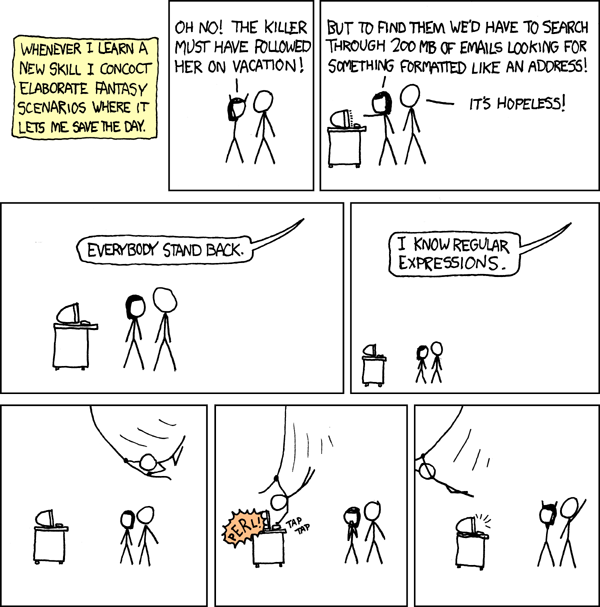
\includegraphics[height=0.8\textheight]{images/regular_expressions.png}\end{center}
\end{frame}

\frame{
  \frametitle{Lizenzen}
  \center
  
\includegraphics[width=2em]{images/by}
  
\includegraphics[width=2em]{images/cc}
  
\includegraphics[width=2em]{images/sa}
  \\
  {\tiny

Dieses Werk ist unter einem ``Creative Commons Namensnennung-Weitergabe unter gleichen Bedingungen 3.0 Deutschland``-Lizenzvertrag lizenziert. Um eine Kopie der Lizenz zu erhalten, gehen Sie bitte zu \href{http://creativecommons.org/licenses/by-sa/3.0/de/}{http://creativecommons.org/licenses/by-sa/3.0/de/} oder schreiben Sie an Creative Commons, 171 Second Street, Suite 300, San Francisco, California 94105, USA.\\
  \vspace{1cm}
  Davon ausgenommen sind das Titelbild, welches aus der März-April 2002 Ausgabe von American Scientist erschienen ist und ohne Erlaubnis verwendet wird, sowie das KIT Beamer Theme. Hierfür gelten die Bestimmungen der jeweiligen Urheber.
  \vspace{1cm}
  \\ 
  }
  %Habe hier die Reihenfolge etwas umgestellt, weil die Formatierung bei mir komisch aussah. 
  %Wenn es bei dir anders ist, kannst du es auch wieder zurückändern, dann haben wir unterschiedliche Kompilieroptionen
}

\end{document}
